\section*{Lectura 8: Espacios Contractibles y Convexidad.}

\begin{definition}
    Un subconjunto $X$ de $\R^n$ se llama \textbf{convexo} s\'i para todo puntos
    $x,y \in X$, la recta trazada entre $x$ y  $y$ esta contenido en  $X$. Es
    decir, que para todo  $t \in [0,1]$, $(1-t)x+ty \in X$.
\end{definition}

\begin{figure}[h]
    \centering
    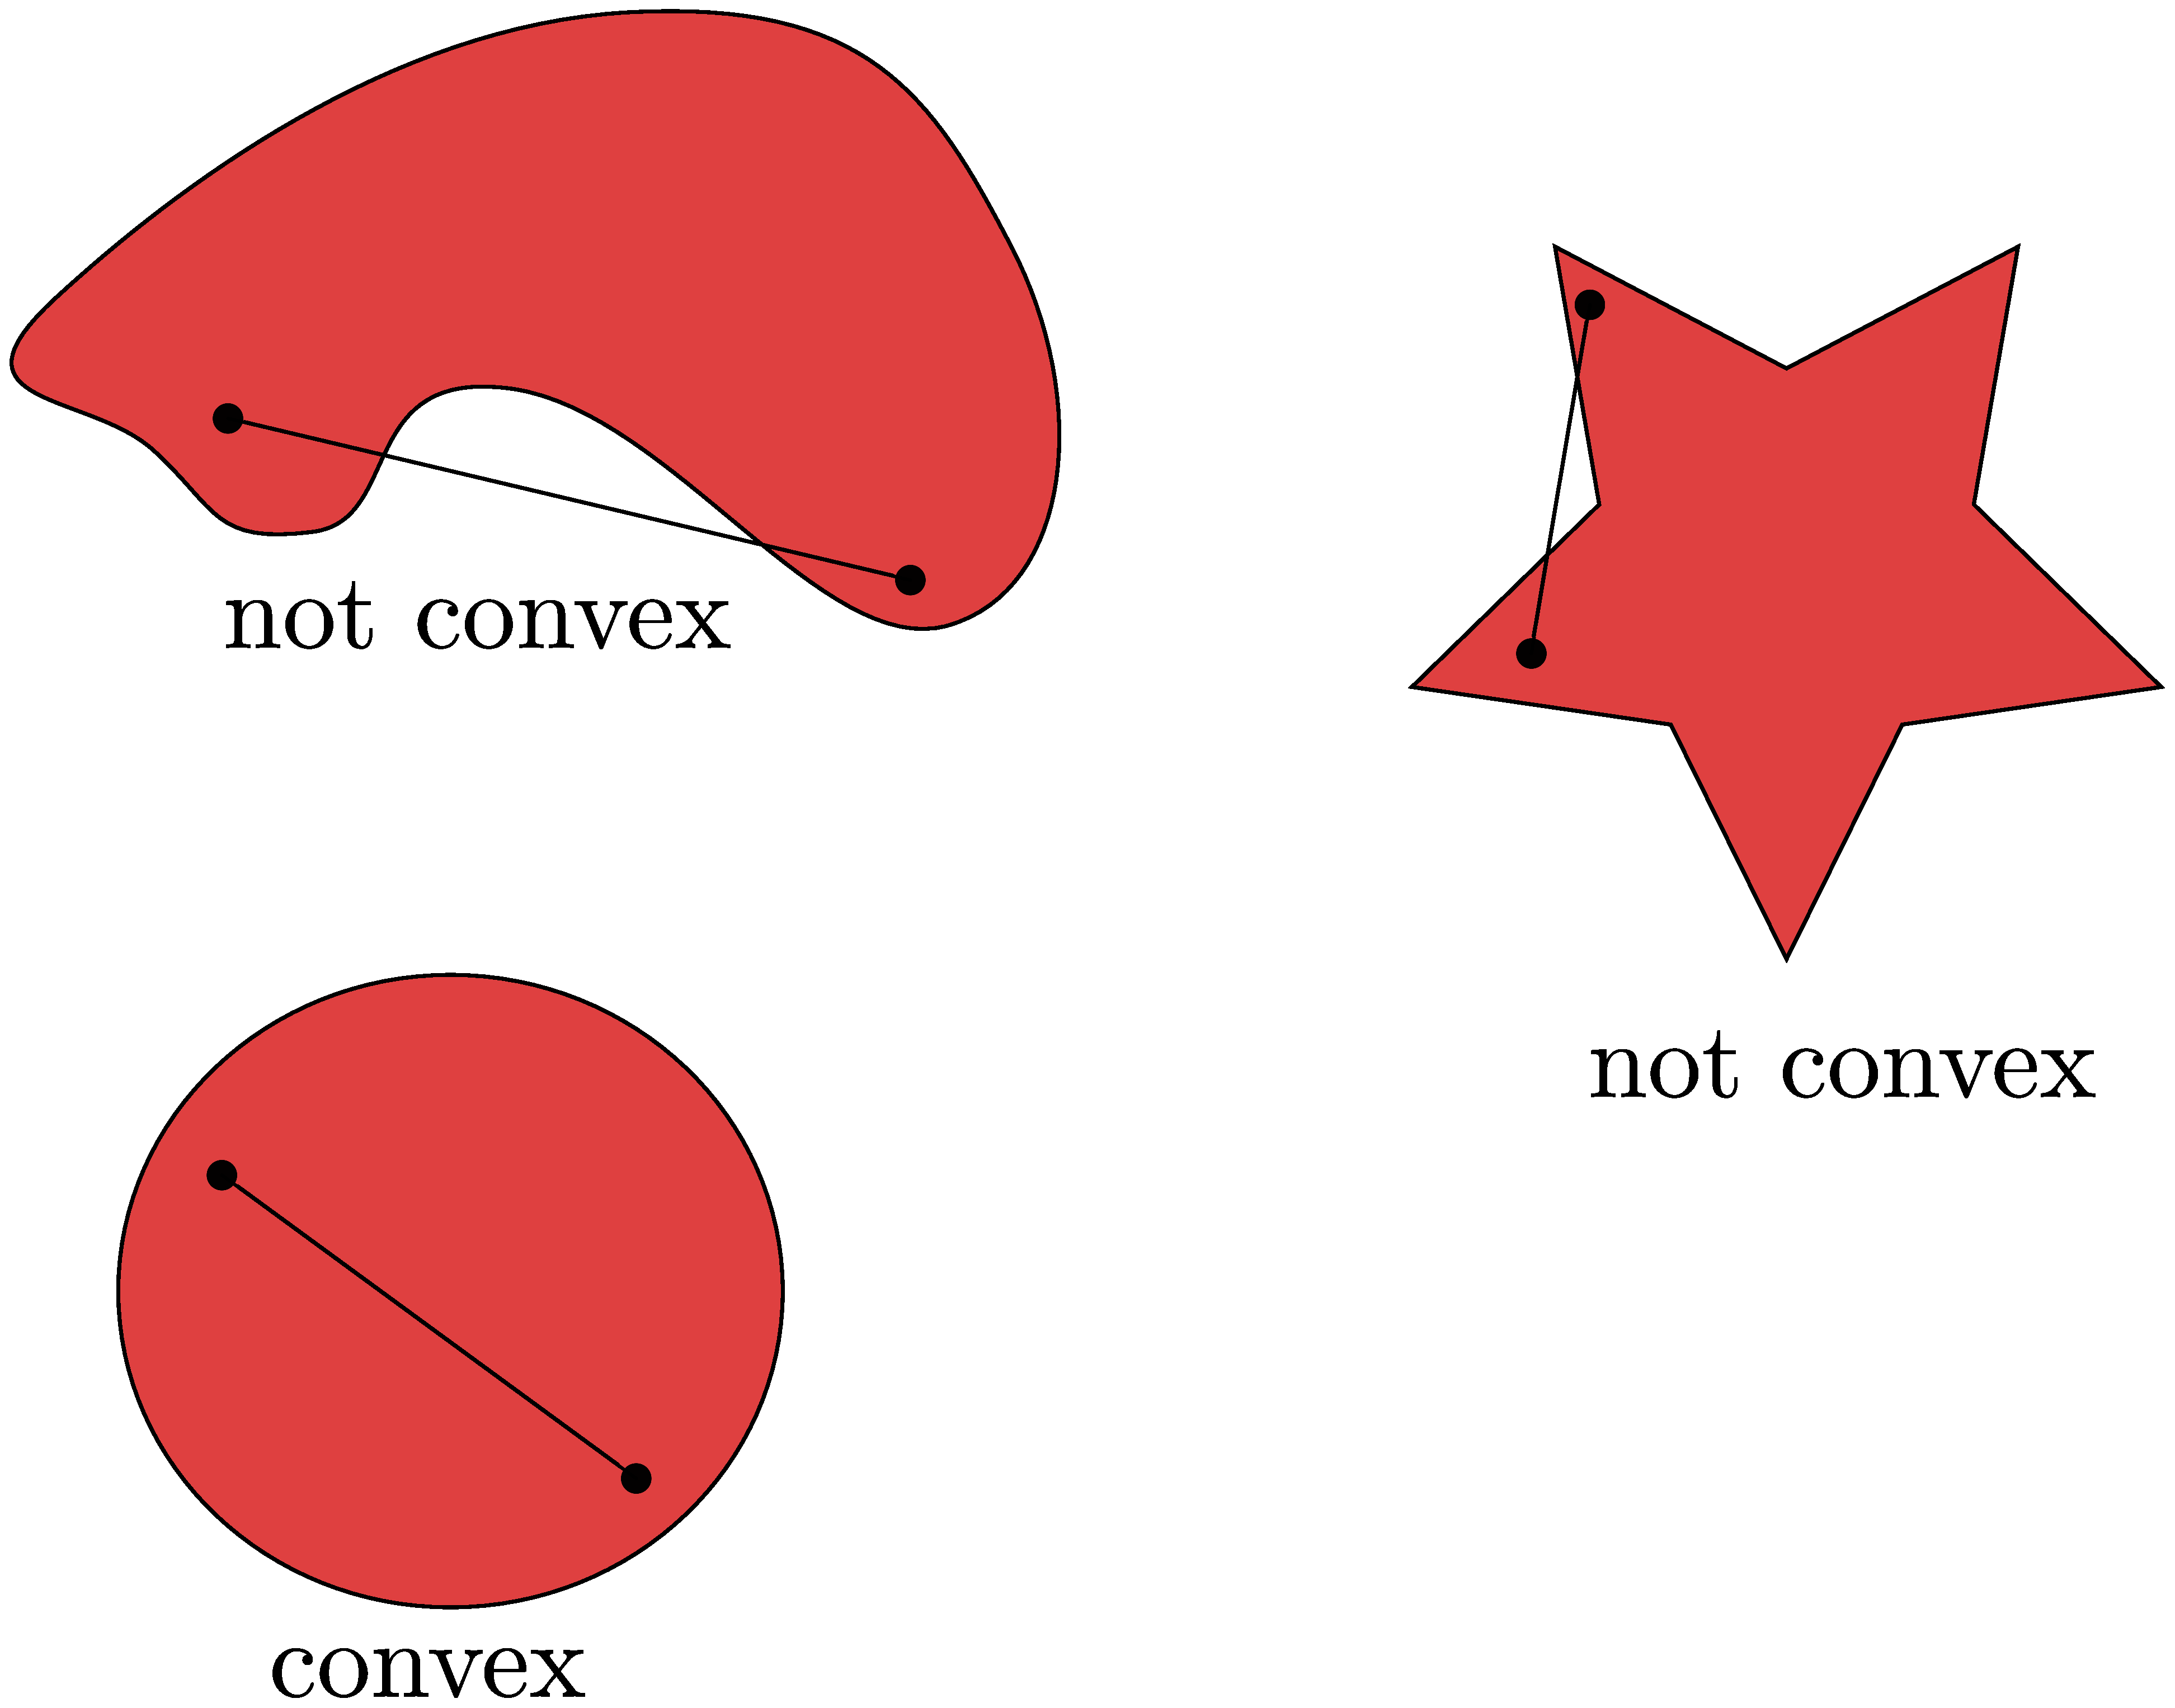
\includegraphics[scale=0.1]{Figures/convex.eps}
    \caption{Espacios convexos y no convexos en $\R^n$. Nota que las estrellas
    no son convexos, pero el disco si es convexo.}
    \label{fig_18}
\end{figure}

\begin{definition}
    Llamamos a un espacio topologico $X$  \textbf{contractible} s\'i la
    identidad en $1_X$ es homotopicamente nula.
\end{definition}

\begin{lemma}\label{lemma_8.13}
    Espacios convexos son contractibles.
\end{lemma}

\begin{example}\label{}
    \begin{enumerate}
        \item[(1)] El disco $D^n$ es contracible como es convexo, pero la esfera
            $S^{n-1}$ no es contractible como $1_{S^{n-1}}$ no puede ser
            homotopicamente nula.

        \item[(2)] EL hemisferio norte de $S^{n-1}$, $H^+=\{x \in S^{n-1} :
            x_{n-1}=0\}$ es contractible, pero no convexo. S\'i una considere
            los geodesicos sobre $H^+$ como las rectas, entonces resulta que
            s\'i  $H^+$ es convexo.
    \end{enumerate}
\end{example}

\begin{definition}
    Sea $X$ un espacio topologico y $X'$ una partici\'on de $X$ en conjuntos
    disjuntos  $X_\alpha$. Definimos la  \textbf{aplicaci\'on canonica} de $X$
    sobre  $X'$ de ser la mapa $q:X \xrightarrow{} X'$ tal que $q:x \xrightarrow{}
    X_\alpha$ s\'i $x \in X_\alpha$.
\end{definition}

\begin{definition}
    Sea $X$ un espacio topologico,  $X'$ una partici\'on de  $X$, y  $q:X
    \xrightarrow{} X'$ la aplicaci\'on canonica de $X$ sobre $X'$. Definimos el
    \textbf{topologia cociente} de $X'$ de ser la colecci\'on
    \begin{equation*}
        \Tc=\{U \subseteq X' : \inv{q}(U) \text{ es abierto en } X\}
    \end{equation*}
    Llamamos a $X'$ bajo este topologia el  \textbf{espacio cociente} de $X$.
\end{definition}

\begin{lemma}\label{lemma_8.14}
    S\'i $X$ es un espacio topologico, y  $X'$ es su espacio cociente, entonces
    la aplicaci\'on canonica de  $X$ sobre  $X'$ es continua. Es decir que $q
    \in \Hom{(X,X')}$ en la categoria $\Top$.
\end{lemma}

\begin{definition}
    Sea $X$ un espacio topologico y  $A \subseteq A$. Defina
    $\faktor{X}{A}=\{A\} \cup \{y \in X : y \notin A\}$. Se llama a
    $\faktor{X}{A}$ bajo el topolog\'ia cociente el \textbf{espacio cociente} de
    $X$  \textbf{colapsada} por $A$. Decimos que $A$ \textbf{colapsa} a un punto
    bajo la topologia cociente.
\end{definition}

\begin{example}\label{}
    S\'i $X=[0,1]$ y $A=\{0,1\}$, entonces el espacio cociente $\faktor{X}{A}
    \simeq S^1$ es homeomorfo al circulo. Se mostra de como se puede llegar de
    $[0,1]$ hasta $S^1$ en el figura \ref{fig_19}.

    \begin{figure}[h]
        \centering
        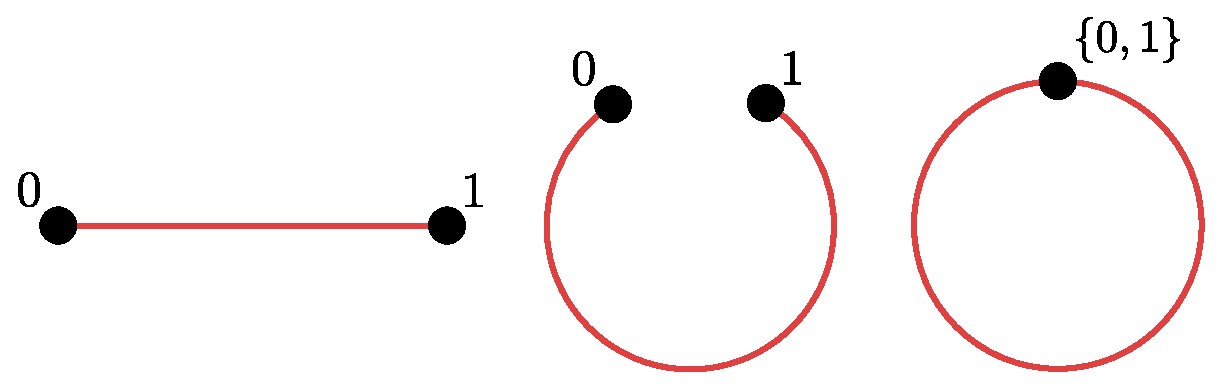
\includegraphics[scale=0.5]{Figures/interval_to_circle.eps}
        \caption{Se puede pensar en la aplicaci\'on canonica de
            $\faktor{[0,1]}{\{0,1\}}$ de coger el intervalo $[0,1]$ y
        deformandolo hasta que pegas el punto $0$ con el punto $1$. El espacio
        resultante es $S^1$.}
        \label{fig_19}
    \end{figure}
\end{example}
